\documentclass[a4paper]{article}
\usepackage{ulem}
\usepackage{setspace}
\usepackage{wrapfig}
\usepackage{bpchem}
\usepackage{color}
\usepackage{subfigure}
\usepackage{float}
\usepackage{titletoc}
\usepackage{indentfirst}
\usepackage{geometry}
\usepackage{amsmath}
\usepackage{amssymb}
\usepackage{graphicx}
\usepackage{enumerate}
\usepackage{url}
\usepackage{caption2}
\usepackage{graphicx}  
\usepackage{epstopdf}
\usepackage{listings}
\lstloadlanguages{[5.2]Mathematica}

\geometry{a4paper,left=2.54cm,right=2.54cm,top=2.54cm,bottom=2.54cm}

\begin {document}
\begin{large}
	\begin{center}
	~\\ ~\\ ~\\ ~\\ ~\\ ~\\ \rule[-1pt]{10.3cm}{0.05em} \\~\\UM-SJTU JOINT INSTITUTE\\~\\Probabilistic Methods in
Engineering\\~\\(VE401)	~\\ \rule[-1pt]{10.3cm}{0.05em} \vspace{7cm} \\Term Project 2
	\end{center}
\end{large}
~\\

\begin{large}
	\begin{center}
	Police Shootings in the United States
	\end{center}
\end{large}
\vspace{5cm}

\begin{tabular}{l l l}
	Name: Feitong Tang&ID: 518370910017&Group 1\\
	Name: Weikai Zhou&ID: 518021911039&Group 1\\
     ~\\
	Date: 30 April 2020
\end{tabular}

\newpage












\section{Abstract}
	Based on David Spiegelhalter and Arthur Barnett's \textit{London murders: a predictable pattern?}, this project analyzes the pattern of occurrence of fatal police shootings in the United States. The project gets its data from the database of the Washington Post and gives an overview of the data. It uses goodness-of-fit test to check whether the occurrence of fatal police shootings in the United States follows a Poisson distribution in the years 2015-2019 and 2020 respectively. It also tests whether the average number of police shootings depends on weekdays. It gives the confidence interval for the parameter $k$ of a Poisson distribution and uses the data from 2015 to 2019 as an example to calculate such confidence interval. It also derives the Nelson prediction interval to predict the future counts of a Poisson distribution and gives the 95\% prediction interval for the number of fatal police shootings in 2020. Finally, it analyzes how COVID-19 will influence the data for 2020.
\\

\noindent\textbf{Keywords}: Fatal police shooting in the United States, Poisson distribution, goodness-of-fit test, confidence interval, prediction interval, COVID-19.



\newpage

\tableofcontents

\newpage

















\section{Introduction}
	\subsection{Background}
	David Spiegelhalter and Arthur Barnett analyzed the pattern of London murders between Apr. 2004 and Mar. 2007, and predicted the number of murders in London during 2008 [1]. Based on their analysis and the data of fatal police shootings in the USA provided by Washington Post [2], we want to analyze the pattern of fatal police shootings in the USA from Jan. 2015, and predict the number of fatal police shootings in 2020.

	\subsection{Objectives}
	\begin{itemize}
	\item Give an overview of the data of fatal police shootings;
	\item Figure out the pattern of fatal police shootings and its dependence on weekday;
	\item Calculate the confidence interval for the parameter of a Poisson distribution;
	\item Predict the numbers of fatal police shootings in 2020;
	\end{itemize}

















\section{Data analysis}
	\subsection{Data source}
	The data we use is based on the database of Washington Post. It records every fatal shooting “in which a police officer, in the line of duty, shoots and kills a civilian” since Jan. 1, 2015. This sentence gives the clear definition of “fatal police shooting”, meaning that the database of Washington Post will not document the deaths of those in custody, fatal shootings by officers who are not on duty and non-shooting deaths. Moreover, the Washington Post gets their information mainly from “news accounts, social media postings and police reports”. It also monitors other database like Killed by Police and Fatal Encounters and updates the database regularly with new fatal police shootings and new facts. Therefore, compared with the database of the FBI and the Centers for Disease Control and Prevention, it is more complete [3].

	\subsection{Overview of the data}
	With the help of Mathematica, we can convert the data from Jan. 1, 2015 to Dec. 31, 2019 into a more comprehensible figure, which shows the number of fatal police shootings on each day (Figure 1).
	
	\begin{figure}[H]
	\centering
	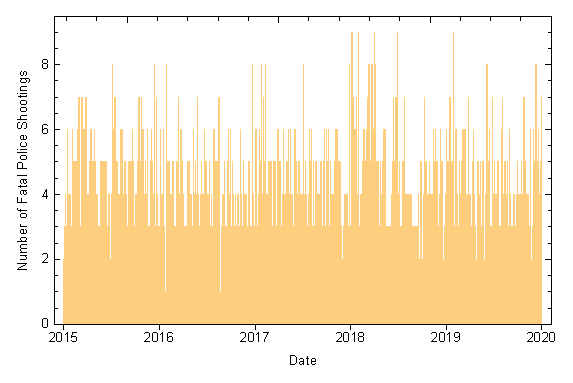
\includegraphics[height=7cm,width=14cm]{Overall(2).eps}
	\caption{Number of fatal police shootings each day from Jan. 1, 2015 to Dec. 31, 2019.}
	\end{figure}

	We notice that there are five days with 9 fatal police shootings recorded and four of them happened in 2018.

















\section{Goodness-of-fit test for Poisson distribution}
	\subsection{Test for 2015-2019}
	In \textit{London murders: a predictable pattern?}, David Spiegelhalter and Arthur Barnett assumed that “if murders happened as random events, the number of murders each day would follow a Poisson distribution” [1]. Similarly, we may assume that the fatal police shootings happened as random events, and the number of fatal police shootings would also follow a Poisson distribution. In order to confirm our assumption, we will test whether the occurrence of fatal police shootings in the USA follows a Poisson distribution or not from 2015 to 2019. From the data, we get the following table (Table 1).

\begin{table}[H]
\centering
\begin{tabular}{|c|c|c|c|c|c|c|c|c|c|c|}
\hline
\begin{tabular}[c]{@{}c@{}}Number of fatal police \\ shootings in a day\end{tabular} & 0   & 1   & 2   & 3   & 4   & 5   & 6  & 7  & 8  & 9 \\ \hline
Observed days                                                                    & 139 & 348 & 414 & 382 & 280 & 151 & 66 & 28 & 13 & 5 \\ \hline
\end{tabular}
\caption{Observed days with different numbers of fatal police shootings.}
\end{table}

	Let $X$ denotes the number of fatal police shootings in a day, then the estimator for $k$ is the sample mean [4], 
\begin{equation}
\begin{split}
\hat{k}=\bar{X}&= \frac{1}{5\cdot365+1} (139\cdot0+348\cdot1+414\cdot2+382\cdot3+ \\  & \quad \   280\cdot4+151\cdot5+66\cdot6+28\cdot7+13\cdot8+5\cdot9) \\
&=2.7043.
\nonumber
\end{split}
\end{equation}

	Then, in order to use the multinomial distribution, we should calculate 
\begin{equation}
\begin{split}
&P[X=0]=\frac{e^{-\hat{k}}{\hat{k}}^0}{0!}=0.0669; \qquad \qquad \qquad P[X=1]=\frac{e^{-\hat{k}}{\hat{k}}^1}{1!}=0.1810;  \\
&P[X=2]=\frac{e^{-\hat{k}}{\hat{k}}^2}{2!}=0.2447; \qquad \qquad \qquad P[X=3]=\frac{e^{-\hat{k}}{\hat{k}}^3}{3!}=0.2206;  \\
&P[X=4]=\frac{e^{-\hat{k}}{\hat{k}}^4}{4!}=0.1491; \qquad \qquad \qquad P[X=5]=\frac{e^{-\hat{k}}{\hat{k}}^5}{5!}=0.0807;  \\
&P[X=6]=\frac{e^{-\hat{k}}{\hat{k}}^6}{6!}=0.0364; \qquad \qquad \qquad P[X=7]=\frac{e^{-\hat{k}}{\hat{k}}^7}{7!}=0.0140;  \\
&P[X=8]=\frac{e^{-\hat{k}}{\hat{k}}^8}{8!}=0.0047;\\
&P[X\ge9]=1-P[X=0]-P[X=1]-\cdots-P[X=8]=0.0019.
\nonumber
\end{split}
\end{equation}

	Therefore, the distribution of $X$ can be expressed as a new distribution with a categorical random variable with parameters $(p_0,\,p_1,\,\cdots,\,p_9)=(0.0669,\, 0.1810,\,\cdots,\,0.0019)$.

	After that, we need to calculate the expected days with $E_i=np_i$, where $i$ is the category and $n$ is the sample size $n=5\cdot365+1=1826$.
\begin{equation}
\begin{split}
&E_0=1826\cdot0.0669=122.19; \qquad \qquad \qquad E_1=1826\cdot0.1810=330.45;  \\
&E_2=1826\cdot0.2447=446.81; \qquad \qquad \qquad E_3=1826\cdot0.2206=402.76;  \\
&E_4=1826\cdot0.1491=272.30; \qquad \qquad \qquad E_5=1826\cdot0.0807=147.27;  \\
&E_6=1826\cdot0.0364=66.38; \qquad \qquad \qquad \,\, \, E_7=1826\cdot0.0140=25.64;  \\
&E_8=1826\cdot0.0047=8.67; \qquad \qquad \qquad\,\, \,\,\, \, E_9=1826\cdot0.0019=3.47.
\nonumber
\end{split}
\end{equation}

	Besides, we should pay attention to the Cochran's Rule, which requires that
\begin{equation}
\begin{split}
&{\rm E}[X_i]=np_i\ge1\qquad \qquad {\rm for\ all}\ i=1,\,\cdots,\,k,\\
&{\rm E}[X_i]=np_i\ge5\qquad \qquad {\rm for\ 80\% \ of\ all}\ i=1,\,\cdots,\,k.
\nonumber
\end{split}
\end{equation}

	We find that all of the $E_i$s are greater than 1 and only one out of ten that is smaller than 5, which means 90\% of the $E_i$s are greater than 5. Therefore, it satisfies the Cochran's Rule, and we can create the following table and figure (Table 2, Figure 2).

\begin{table}[H]
\centering
\setlength{\tabcolsep}{1.5mm}{
\begin{tabular}{|c|c|c|c|c|c|c|c|c|c|c|}
\hline
\begin{tabular}[c]{@{}c@{}}Number of fatal police \\ shootings in a day\end{tabular} & 0      & 1      & 2      & 3      & 4      & 5      & 6     & 7     & 8    & 9    \\ \hline
Expected days                                                                        & 122.19 & 330.45 & 446.81 & 402.76 & 272.30 & 147.27 & 66.38 & 25.64 & 8.67 & 3.47 \\ \hline
Obseved days                                                                         & 139    & 348    & 414    & 382    & 280    & 151    & 66    & 28    & 13   & 5    \\ \hline
\end{tabular}}
\caption{Expected and observed days with different numbers of fatal police shootings.}
\end{table}

\begin{figure}[H]
\centering
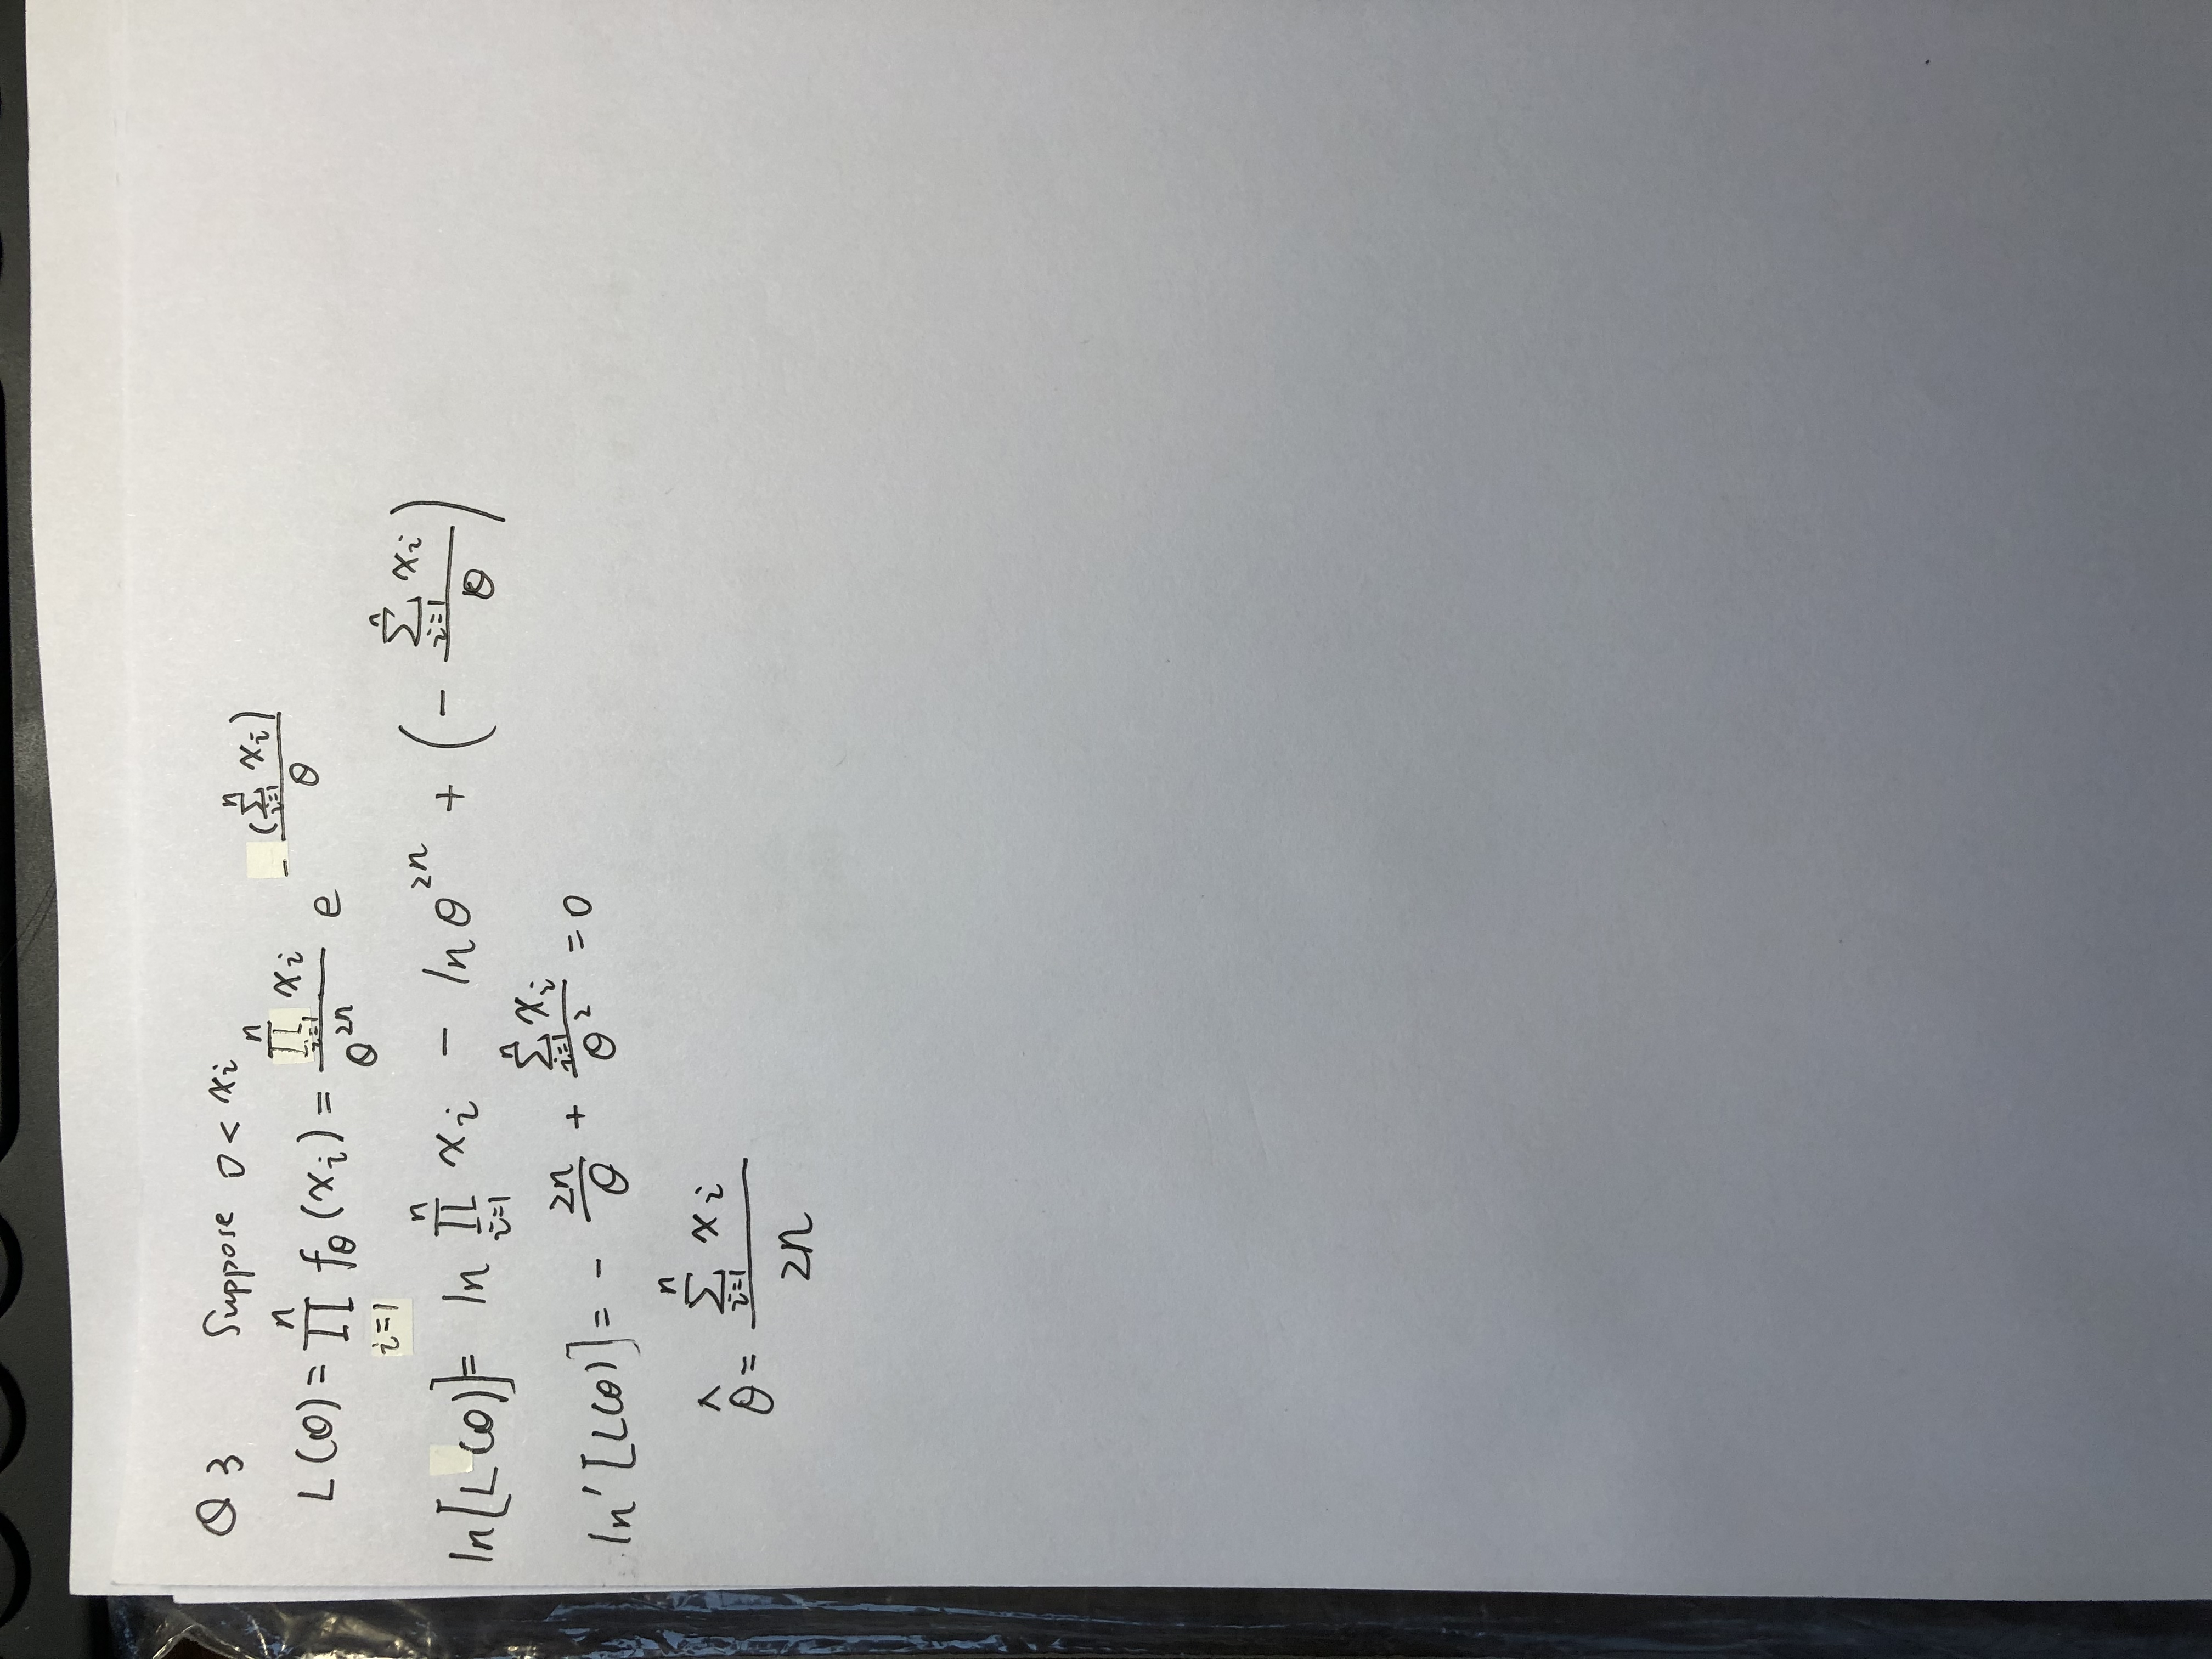
\includegraphics[height=5cm,width=15cm]{3.eps}
\captionsetup{justification=centering}
\caption{Days with different numbers of fatal police shootings: (a) expected; (b) observed.}
\end{figure}

	Then, the hypothesis “$H_0$: the number of fatal police shootings follows a Poisson distribution with parameter $k=2.7043$” is equivalent to “$H_0$: the number of fatal police shootings follows a multinomial distribution with parameters $(0.0669,\, 0.1810,\,\cdots,\,0.0019)$”. Besides, $$X^2=\sum_{i=1}^N\frac{(O_i-E_i)^2}{E_i}$$ follows a chi-squared distribution with $N-1-m=10-1-1=8$ degree of freedom, where $O_i$ is the observed value and $m$ is the number of parameters that we estimate. After we plug in the number, we get $X^2=10.94$. Let $\alpha=0.05$, we have $\chi_{0.05,\,8}^2=15.51>10.94$. Therefore, we are unable to reject $H_0$ at the 5\% level of significance. We can calculate the $P$-value as follows $$P=P[X^2|H_0]\le P[\chi_8^2\ge10.94]=1-P[\chi_8^2\le10.94]=1-0.7949=0.2051.$$The $P$-value is quite large; therefore, we cannot reject $H_0$, and we should consider that the number of fatal police shootings during Jan. 1, 2015 and Dec. 31, 2019 follows a Poisson distribution with parameter $k=2.7043$ [5].






\subsection{Test for 2020}

    Similarly, we want to test whether the number of murders each day from Jan. to Apr. 15, 2020 follows a Poisson distribution. From the data, we can get the following table (Table 3).

\begin{table}[H]
\centering
\begin{tabular}{|c|c|c|c|c|c|c|c|c|c|}
\hline
\begin{tabular}[c]{@{}c@{}}Number of fatal police \\ shootings in a day\end{tabular} & 0   & 1   & 2   & 3   & 4   & 5   & 6  & 7  & 8   \\ \hline
Observed days                                                                    & 7 & 18 & 27 & 18 & 14 & 13 & 8 & 0 & 1  \\ \hline
\end{tabular}
\caption{Observed days with different numbers of fatal police shootings.}
\end{table}

	Then, we use the unbiased estimator $\bar{X}$ to estimate the parameter $k$. Based on the available data, we have: $$\hat{k}_{2020}=\bar{X}=\frac{303}{106}=2.8585.$$
    
    Then we can calculate the expected probability to use the multinomial distribution.
\begin{equation}
\begin{split}
&P[X=0]=\frac{e^{-\hat{k}}{\hat{k}}^0}{0!}=0.0574; \qquad \qquad \qquad P[X=1]=\frac{e^{-\hat{k}}{\hat{k}}^1}{1!}=0.1639;  \\
&P[X=2]=\frac{e^{-\hat{k}}{\hat{k}}^2}{2!}=0.2343; \qquad \qquad \qquad P[X=3]=\frac{e^{-\hat{k}}{\hat{k}}^3}{3!}=0.2233;  \\
&P[X=4]=\frac{e^{-\hat{k}}{\hat{k}}^4}{4!}=0.1596; \qquad \qquad \qquad P[X=5]=\frac{e^{-\hat{k}}{\hat{k}}^5}{5!}=0.0912;  \\
&P[X=6]=\frac{e^{-\hat{k}}{\hat{k}}^6}{6!}=0.0435; \qquad \qquad \qquad P[X=7]=\frac{e^{-\hat{k}}{\hat{k}}^7}{7!}=0.0177;  \\
&P[X\ge8]=1-P[X=0]-P[X=1]-\cdots-P[X=7]=0.0091.
\nonumber
\end{split}
\end{equation}
    
	Then, we calculate the expected days respectively.
\begin{equation}
\begin{split}
&E_0=106\cdot0.0574=6.08; \qquad \qquad \qquad E_1=106\cdot0.1639=17.38;  \\
&E_2=106\cdot0.2343=24.84;\qquad \qquad \,\,\,\,\,\,\,\,\, E_3=106\cdot0.2233=23.67;  \\
&E_4=106\cdot0.1596=16.91;\qquad \qquad \,\,\,\,\,\,\,\,\, E_5=106\cdot0.0912=9.67;  \\
&E_6=106\cdot0.0435=4.61;\qquad \qquad \,\,\,\,\,\,\,\,\,\,\,\, E_7=106\cdot0.0177=1.88;  \\
&E_8=106\cdot0.0091=0.97.  
\nonumber
\end{split}
\end{equation}    
    
	Besides, we notice that it does not satisfy the Cochran's Rule since $E_8<1$ and $E_6,\, E_7 <5$. Thus, we combine the last three categories together and create the following table (Table 4).
\begin{table}[H]
\centering
\setlength{\tabcolsep}{1.5mm}{
\begin{tabular}{|c|c|c|c|c|c|c|c|}
\hline
\begin{tabular}[c]{@{}c@{}}Number of fatal police \\ shootings in a day\end{tabular} & 0      & 1      & 2      & 3      & 4      & 5      & 6 or more             \\ \hline
Expected days                                                                        & 6.08 & 17.38 & 24.84 & 23.67 & 16.91 & 9.67 & 7.46  \\ \hline
Obseved days                                                                         & 7    & 18    & 27    & 18    & 14    & 13    & 9       \\ \hline
\end{tabular}}
\caption{Expected and observed days with different numbers of fatal police shootings.}
\end{table}
	Then, the hypothesis “$H_0$: the number of fatal police shootings from Jan. 1 to Apr. 15, 2020 follows a Poisson distribution with parameter $k$ = 2.8585” is equivalent to “$H_0$: the number of fatal police shootings from Jan. 1 to Apr. 15, 2020 follows a multinomial distribution with parameters (0.0574, 0.1639, $\cdots$ , 0.0703)”. Besides, $$X^2=\sum\limits_{i=1}^7\frac{(O_i-E_i)^2}{E_i}=\frac{(7-6.08)^2}{6.08}+\cdots+\frac{(9-7.46)^2}{7.46}=3.67$$ follows a chi-squared distribution with $N-1-m=7-1-1=5$ degrees of freedom. For $\alpha=0.05$, $\chi^2_{0.05,\,5}=11.07>3.67$. Therefore, we are unable to reject $H_0$ at the 5\% level of significance. The result shows that the data from Jan. 1 to Apr. 15, 2020 follows a Poisson distribution [5].





















\section{Dependence on weekday}
	From the data of 2015-2019, we can also create the following figures that shows the number of fatal police shootings on each weekday and month (Figure 3).
\begin{figure}[H]
\centering
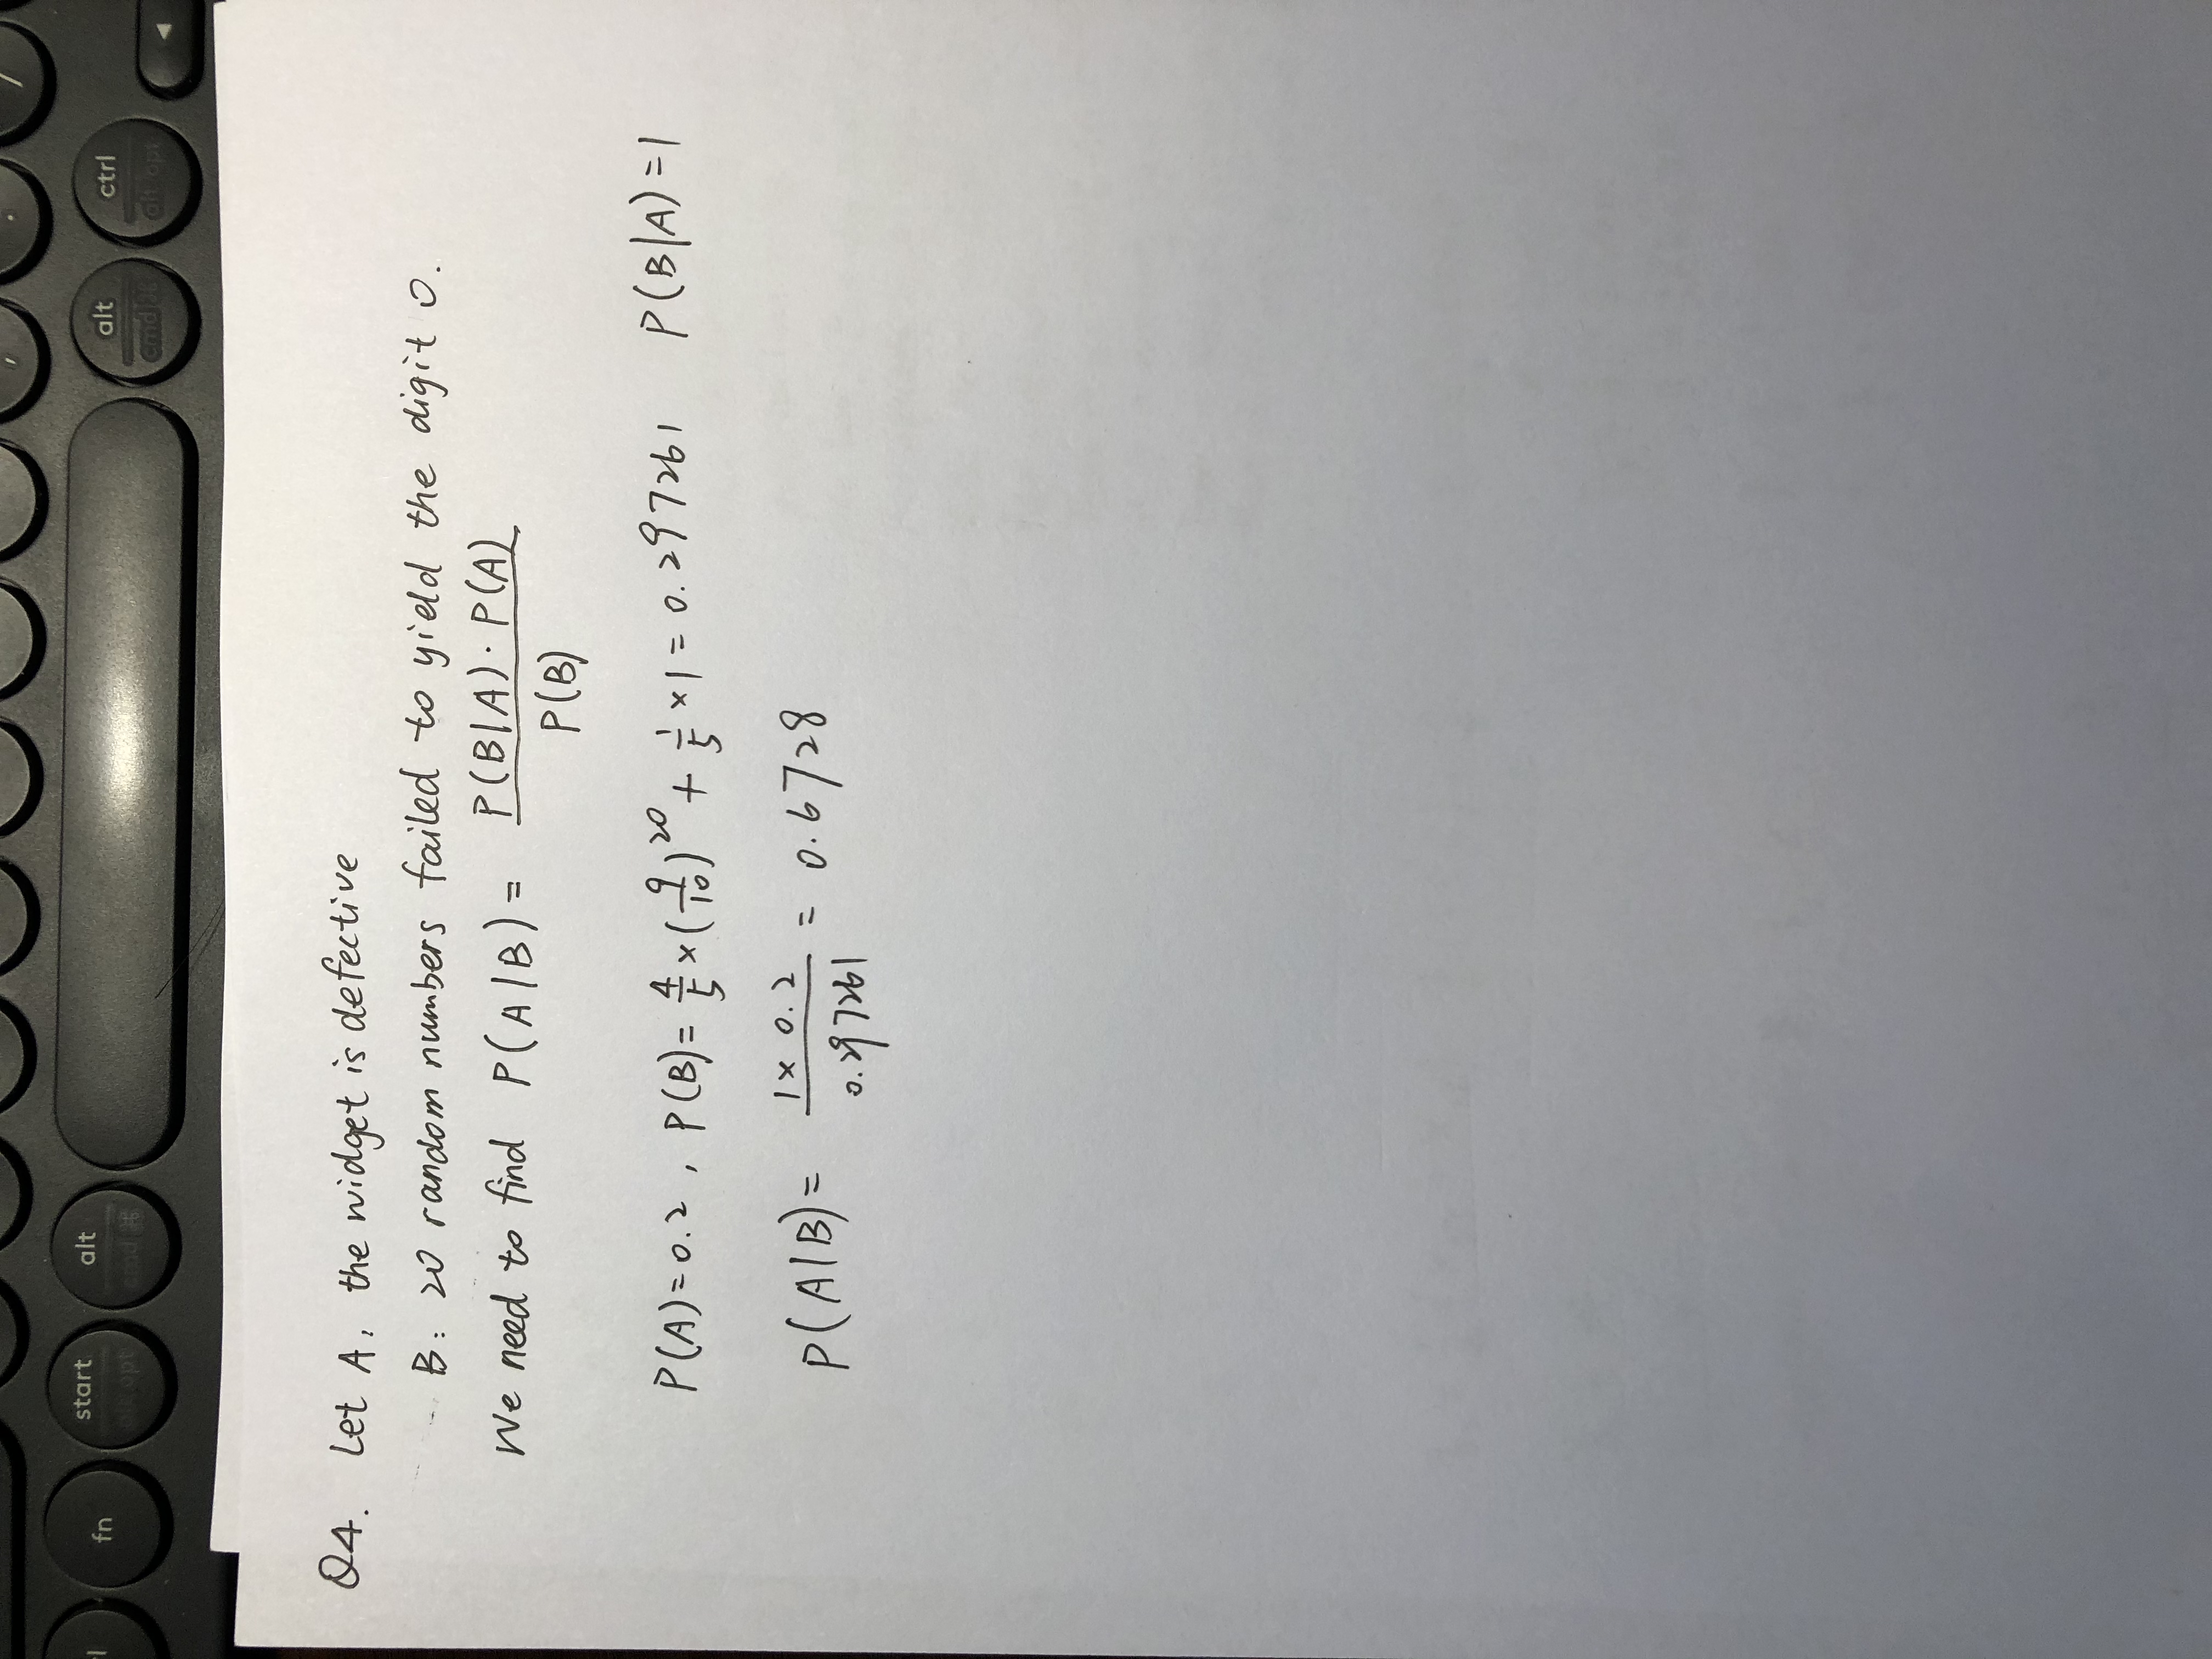
\includegraphics[height=4cm,width=13cm]{4.eps}
\captionsetup{justification=centering}
\caption{Number of occurrence of police shootings on (a) different weekdays and (b) different months.}
\end{figure}

We want to test whether there is evidence that the average number of police shootings depends on the weekday, then we should set the null hypothesis as “$H_0$: the number of fatal police shootings follows a multinomial distribution with the same parameter $p=\frac{1}{7}$” because there are seven different weekdays. There are 4938 fatal police shootings in total, so we can calculate the expected value on each weekday:
$$E_i=np_i=4938\times\frac{1}{7}=705.43.$$
Then we can get the following table (Table 5).
\begin{table}[H]
\centering
\begin{tabular}{|c|c|c|c|c|c|c|c|}
\hline
Weekdays         & Mon.   & Tue.   & Wed.   & Thu.  & Fri.   & Sat.   & Sun.   \\ \hline
Expected numbers & 705.43 & 705.43 & 705.43 & 705.43 & 705.43 & 705.43 & 705.43 \\ \hline
Obseved numbers  & 668    & 742    & 757    & 732    & 692    & 662    & 685    \\ \hline
\end{tabular}
\caption{Expected and observed number of fatal police shootings on different weekdays.}
\end{table}

We notice that it satisfies the Cochran's Rule because all the $E_i$s are greater than 5. Therefore,
$$X^2=\sum_{i=1}^7\frac{(O_i-E_i)^2}{E_i}=\frac{(668-705.43)^2}{705.43}+\cdots+\frac{(685-705.43)^2}{705.43}=12.17$$ follows a chi-squared distribution with $N-1-m=7-1-0=6$ degree of freedom. Let $\alpha=0.05$, we have $\chi_{0.05,\,6}^2=12.59>12.17$. Therefore, we fail to reject $H_0$ at the 5\% level of significance, which means we can consider that the occurrence of fatal police shootings is independent on weekdays [5].

























\section{Confidence interval for the parameter of Poisson distribution}
	\subsection{General confidence interval for the parameter of Poisson distribution}
	Let $X_1$, $X_2$, ..., $X_n$ be a random sample of size $n$ from a Poisson distribution with parameter $k$, mean $\mu$ and variance $\sigma^2$. For Poisson distribution, we have $\mu=k$ and $\sigma^2=k$ and we've already proved that the unbiased estimator for the parameter $k$ is $\hat{k}=\bar{X}$ [4]. And for a large sample size $n$, we can assume that $\bar{X}$ approximately follows a normal distribution with mean $\mu$ and variance $\sigma^2/n$ [4]. Then, $$\frac{\bar{X}-\mu}{\sigma/\sqrt{n}}=\frac{\hat{k}-k}{\sqrt{k/n}}$$ is approximately standard-normally distributed.

	The $100(1-\alpha)\%$ confidence interval for $k$ is then given as follows [6]: $$\hat{k}\pm z_{\alpha/2}\sqrt{k/n}.$$
	
	But the interval depends on the unknown parameter $k$, which we are currently estimating. We may replace $k$ with $\hat{k}$. Thus we can rewrite the $100(1-\alpha)\%$ confidence interval as $$\hat{k}\pm z_{\alpha/2}\sqrt{\hat{k}/n}.$$ However, $z_{\alpha/2}$ is no longer accurate. But for large sample size $n$, we may consider that the difference between $z_{\alpha/2}$ and the correct value is small enough for us to neglect [7].
	\subsection{Confidence interval for the parameter from 2015-2019}
	Based on the data from 2015 to 2019, we have 4938 fatal police shooting in the total 1826 days. Thus, we have: $$\hat{k}=\bar{X}=\frac{4938}{1826}=2.7043$$

	We use 95\% confidence interval as an example: $$\hat{k}\pm z_{\alpha/2}\sqrt{\hat{k}/n}=2.7043\pm1.96\times\sqrt{2.7043/1826}=2.7043\pm0.0754=[2.6289,\, 2.7797].$$





























\section{Prediction interval for upcoming data}
\subsection{General form of prediction interval}
	According to the article “Improved closed-form prediction intervals for binomial and Poisson distributions”, we can use the Nelson prediction interval to predict the future counts of a Poisson distribution [8].
	
	We will first define some parameters used in calculation: let $\lambda$ be the mean of the Poisson distribution; in the sample size of $n$, there are a total of $X$ existing counts; in another sample size of $m$ of the same Poisson distribution, there will be a total of $Y$ future counts [8].
	
	First, it is easy to find that the estimator $\hat{\lambda}=\bar{X}=X/n$. At the same time, $\hat{\lambda}=\hat{Y}/m$. From these two equations, we have: $$\hat{\lambda}=\frac{X}{n}=\frac{\hat{Y}}{m},\qquad\qquad\qquad\hat{Y}=m\hat{\lambda}=\frac{mX}{n}.$$

Also, to estimate the variance of $m\hat{\lambda}-Y$, we calculate as follows:
\begin{align*}
\hat{\rm Var}(m\hat{\lambda}-Y)&=\hat{\rm Var}(\frac{mX}{n}-Y)\\
&=\frac{m^2}{n^2}\hat{\rm Var}(X)+\hat{\rm Var}(Y)\\
&=\frac{m^2}{n^2}n\hat{\lambda}+m\hat{\lambda}\\
&=m^2\hat{\lambda}(\frac{1}{n}+\frac{1}{m})\\
&=m\hat{Y}(\frac{1}{m}+\frac{1}{n})
\end{align*}

	And the Nelson prediction interval is based on the asymptotic result that $$\frac{m\hat{\lambda}-Y}{\sqrt{\hat{\rm Var}(m\hat{\lambda}-Y})}$$ follows a standard normal distribution [8]. We may calculate the 100(1-$\alpha$)\% prediction interval as follows:
\begin{align*}
1-\alpha&=P\left[-z_{\alpha/2}\le\frac{m\hat{\lambda}-Y}{\sqrt{\hat{\rm Var}(m\hat{\lambda}-Y)}}\le z_{\alpha}\right] \\
&=P\left[-z_{\alpha/2}\sqrt{\hat{\rm Var}(m\hat{\lambda}-Y)}\le m\hat{\lambda}-Y\le z_{\alpha/2}\sqrt{\hat{\rm Var}(m\hat{\lambda}-Y)}\right]\\
&=P\left[m\hat{\lambda}-z_{\alpha/2}\sqrt{\hat{\rm Var}(m\hat{\lambda}-Y)}\le Y\le m\hat{\lambda}+z_{\alpha/2}\sqrt{\hat{\rm Var}(m\hat{\lambda}-Y)}\right]\\
&=P\left[\hat{Y}-z_{\alpha/2}\sqrt{m\hat{Y}(\frac{1}{m}+\frac{1}{n})}\le Y\le \hat{Y}+z_{\alpha/2}\sqrt{m\hat{Y}(\frac{1}{m}+\frac{1}{n})}\right]
\end{align*}

	From the above formula, we can conclude that 100(1-$\alpha$)\% prediction interval is $$[\lceil L\rceil,\,\lfloor U\rfloor]\quad {\rm with}\quad [L,\, U]=\hat{Y}\pm z_{\alpha/2}\sqrt{m\hat{Y}(\frac{1}{m}+\frac{1}{n})},$$ where $\lceil L\rceil$ means the smallest integer greater than or equal to $L$, and $\lfloor U\rfloor$ means the  largest integer less than or equal to $U$ [8].

\subsection{95\% prediction interval for 2020}
	Based on the data from 2015-2019, we know that $$X=4928,\qquad\qquad\qquad n=1826.$$
	
	We fix $\alpha=0.05$, so $z_{\alpha /2}=1.96$. Then we can use the data to obtain the prediction interval:
	
	$$\frac{mX}{n}\pm z_{\alpha /2}\sqrt{\frac{m^2X}{n}\bigg(\frac{1}{m}+\frac{1}{n}\bigg)}=\frac{4938m}{1826}\pm1.96\times\sqrt{\frac{4938m^2}{1826}\bigg(\frac{1}{m}+\frac{1}{1826}\bigg)}$$
	
	After simplification, we obtain the 95\% prediction interval shown by the following interval: $$[\lceil2.7043m-1.96\sqrt{2.7043m+0.0015m^2}\rceil,\, \lfloor2.7043m+1.96\sqrt{2.7043m+0.0015m^2}\rfloor].$$
	

	Figure 4 shows the predicted number of fatal police shooting in the US during 2020 (black line) and the 95\% prediction limits (blue dash lines) with the data for 2020 so far (red dots).
	
	\begin{figure}[H]
    \centering
    \subfigure[Overview of the whole year]{
	\begin{minipage}[t]{0.47\linewidth}
	\centering
	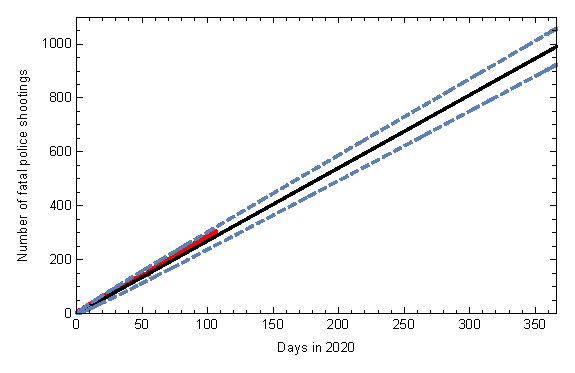
\includegraphics[width=75mm,height=50mm]{prediction_over.eps}
	\end{minipage}
	}
	\subfigure[Detailed for 2020 so far]{
	\begin{minipage}[t]{0.47\linewidth}
	\centering
	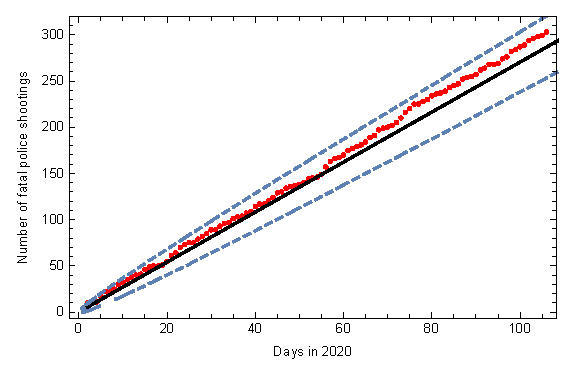
\includegraphics[width=75mm,height=50mm]{prediction_detail.eps}
	\end{minipage}
	}
	\caption{Predicted number of fatal police shootings in 2020 with 95\% prediction limits: (a) overview; (b) detailed.}
    \end{figure}
    
    From Figure 4, we can find that the data for 2020 lies in the prediction interval quite well. This indicates that based on the data for 2015-2019, we can roughly predict the future tendency of the fatal police shooting.























\section{Influence of the outbreak of Coronavirus}

	We must note that the Poisson distribution model is based on the assumption that “the level of violence remains the same” [1]. However, when taking the outbreak of the Coronavirus into account, we should be careful whether this will influence our original assumption.
	
	Before focusing on the influence of the outbreak of COVID-19 on fatal police shooting, we may first have a general idea of the situation of COVID-19 in the US. The following figure (Figure 5) is a screenshot of the number of people confirmed COVID-19 in the US provided by Johns Hopkins University. The marked point is the data for Mar. 27, when the confirmed people first exceeded 100,000 people and reaches around 101,700 people [9].
	
	\begin{figure}[H]
	\centering
	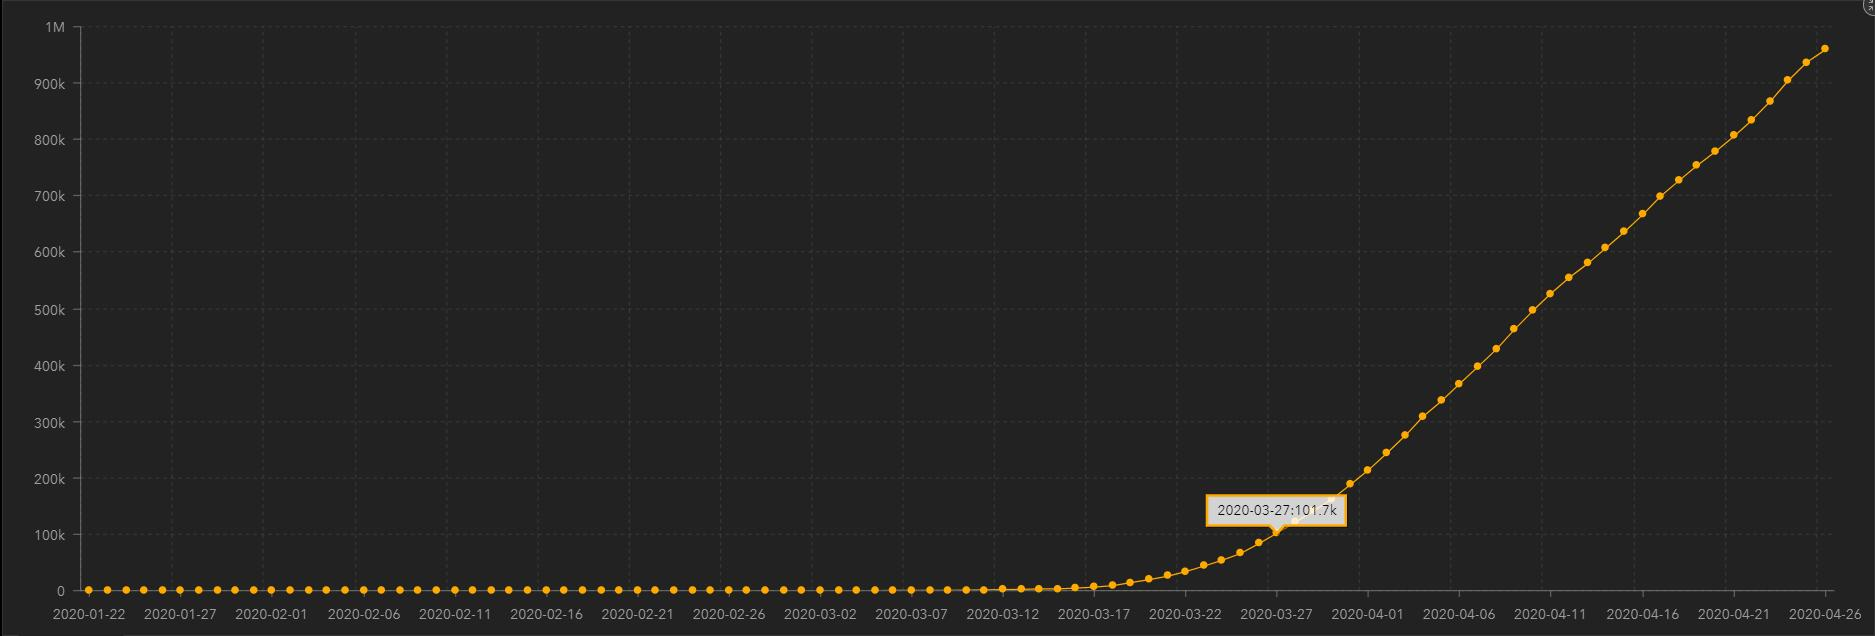
\includegraphics[width=122.2mm,height=45mm]{covid19.jpg}
	\caption{Number of people infectied with COVID-19 in the US [9].}
	\end{figure}
	
	If we look deep into the data, we can find that there's no strong evidence indicating that the outbreak of COVID-19 has a strong influence on the fatal police shooting generally since the previous sections have reached the conclusion that the data for 2020 still follows a Poisson distribution and the data so far all falls in the prediction interval.
	
	However, we may still get some information from the data. If we turn to Figure 4, we may find that for the first half of the data so far, it is really close to the exact predicted line. For the second half of the data, however, the number of fatal police shooting is rising relatively faster and is approaching the upper bound of the prediction interval. The turning point is in March, which is also the time when COVID-19 broke out in the US.
	
	The reason why the number is rising may be due to the following several reasons:
	
	1. The outbreak of COVID-19 makes the residents panic and thus more people are likely to do extreme things including robbing necessities;
	
	2. The US government doesn't respond to the epidemic properly and effectively, leading to some citizens' discontent to the government;

	3. Some residents don't obey the government's control measures and have conflicts with the police.
	
	Besides, if the situation of COVID-19 in the US continues to be worsen in the following months, maybe more people will choose to stay at home. Therefore, the number of fatal police shootings will be reduced.



















\section{Conclusion}
	
	The project mainly analyzes the data of fatal police shooting in the US for 2015-2019 and predict the possible tendency in 2020. We first specify the definition of “fatal police shooting” and give a general overview of the data. We analyze the data for 2015-2019 and 2020 respectively by checking their fitness to the Poisson distribution, the confidence interval of the parameter $k$ of the Poisson distribution and the relationship between fatal police shooting and each weekday. Then we want to predict the data for 2020 based on the previous data and get the 95\% prediction interval for 2020. Finally, we take the outbreak of COVID-19 into account and analyze its influence on number of fatal police shootings.
	
	Through this project, we confirm that the data for fatal police shooting follows a Poisson distribution. Based on the previous data, we can also predict the future possible numbers of fatal police shooting to a certain extent. Moreover, considering the special situation this year, namely the outbreak of COVID-19, it's still not quite clear whether it will significantly influence fatal police shooting.
























\section{Reference}
[1] D. Spiegelhalter and A. Barnett, “\textit{London murders: a predictable pattern?}” Significance, vol. 6, no. 1, pp. 5–8, 2009. \url{http://onlinelibrary.wiley.com/doi/10.1111/j.1740-9713.2009.00334.x/abstract}.

[2] The Washington Post, “\textit{Data-police-shootings},” GitHub. \url{https://github.com/washingtonpost/data-police-shootings}. Accessed April 28, 2020.

[3] The Washington Post, “\textit{Fatal force}.” \url{https://www.washingtonpost.com/graphics/national/police-shootings-2016/}. Accessed April 19, 2020.

[4] H. Hohberger, “\textit{Ve401\_video\_12},” UMJI-SJTU, pp. 18-19, 2020.

[5] H. Hohberger, “\textit{Ve401\_video\_23},” UMJI-SJTU, pp. 9-36, 2020.

[6] H. Hohberger, “\textit{Ve401\_video\_13},” UMJI-SJTU, pp. 8-9, 2020.

[7] H. Hohberger, “\textit{Ve401\_video\_19},” UMJI-SJTU, pp. 4, 2020.

[8] K. Krishnamoorthy and J. Peng, “\textit{Improved closed-form prediction intervals for binomial and Poisson distributions},” Journal of Statistical Planning and Inference, vol. 141, no. 5, pp. 1709-1718, 2011. \url{http://www.sciencedirect.com/science/article/pii/S0378375810005215}.

[9] Johns Hopkins University, “\textit{COVID-19 United States Cases by County},” Coronavirus Resource Center.  \url{https://coronavirus.jhu.edu/us-map}. Accessed April 28, 2020.

\newpage
















\section{Appendix}
	\subsection{Code for Figure 1}
\begin{lstlisting}
data := Import["shootingdata.csv"][[2 ;; 4939, 3]]
DateHistogram[data, "Day", 
 Ticks -> {{"2015", "2016", "2017", "2018", "2019", "2020"}, 
   Automatic}, Frame -> True, 
 FrameLabel -> {"Date", "Number of Fatal Police Shootings"}]
\end{lstlisting}
\

	\subsection{Code for Figure 2}
\begin{lstlisting}
BarChart[{122.19, 330.45, 446.81, 402.76, 272.30, 147.27, 66.38, 
  25.64, 8.67, 3.47}, 
 ChartLabels -> {"0", "1", "2", "3", "4", "5,", "6", "7", "8", 
   "9 or more"}, Frame -> True, 
 FrameLabel -> {"Number of fatal police shootings per day", 
   "Predicted number of occurrences"}, PlotRange -> {0, 450}]

BarChart[{139, 348, 414, 382, 280, 151, 66, 28, 13, 5}, 
 ChartLabels -> {"0", "1", "2", "3", "4", "5,", "6", "7", "8", 
   "9 or more"}, Frame -> True, 
 FrameLabel -> {"Number of fatal police shootings per day", 
   "Actual number of occurrences"}, PlotRange -> {0, 450}, 
 ChartStyle -> Darker[Blue]]
\end{lstlisting}
\

	\subsection{Code for Figure 3}
\begin{lstlisting}
data := Import["shootingdata.csv"][[2 ;; 4939, 3]]
DateHistogram[data, "Day", DateReduction -> "Week", Frame -> True, 
 FrameLabel -> {None, "Number of Fatal Police Shootings"}]
DateHistogram[data, "Month", DateReduction -> "Year", Frame -> True, 
 FrameLabel -> {None, "Number of Fatal Police Shootings"}]
\end{lstlisting}
\

	\subsection{Code for Figure 4}

\begin{lstlisting}
Show[ListPlot[{4, 10, 10, 11, 17, 22, 23, 25, 30, 32, 35, 38, 40, 41, 
   46, 49, 50, 50, 51, 55, 61, 64, 70, 73, 75, 75, 79, 82, 85, 89, 89,
    93, 96, 97, 101, 103, 104, 107, 109, 114, 117, 117, 120, 124, 129,
    130, 134, 136, 137, 138, 140, 144, 145, 146, 149, 157, 163, 166, 
   167, 170, 175, 177, 179, 181, 184, 189, 191, 197, 199, 200, 202, 
   205, 210, 216, 220, 225, 225, 228, 230, 234, 236, 237, 239, 243, 
   245, 247, 252, 254, 255, 257, 262, 264, 268, 268, 269, 274, 276, 
   282, 284, 287, 289, 294, 296, 298, 299, 303}, PlotStyle -> Red, 
  PlotRange -> {{0, 366}, {0, 1100}}, PlotStyle -> SmallCircle, 
  Frame -> True, 
  FrameLabel -> {"Days in 2020", "Number of fatal police shootings"}],
  Plot[2.7043*m, {m, 1, 366}, PlotStyle -> Black, Frame -> Ture, 
  PlotRange -> {{0, 366}, {0, 1100}}, Frame -> True, 
  FrameLabel -> {"Days in 2020", "Number of fatal police shootings"}],
  Plot[Floor[2.7043*m + 1.96*Sqrt[2.7043*m + 0.0015*m^2]], {m, 1, 
   366}, PlotStyle -> Dashed, PlotRange -> {{0, 366}, {0, 1100}}, 
  Frame -> True, 
  FrameLabel -> {"Days in 2020", "Number of fatal police shootings"}],
  Plot[Ceiling[2.7043*m - 1.96*Sqrt[2.7043*m + 0.0015*m^2]], {m, 1, 
   366}, PlotStyle -> Dashed, PlotRange -> {{0, 366}, {0, 1100}}, 
  Frame -> True, 
  FrameLabel -> {"Days in 2020", "Number of fatal police shootings"}]]
  
  Show[ListPlot[{4, 10, 10, 11, 17, 22, 23, 25, 30, 32, 35, 38, 40, 41, 
   46, 49, 50, 50, 51, 55, 61, 64, 70, 73, 75, 75, 79, 82, 85, 89, 89,
    93, 96, 97, 101, 103, 104, 107, 109, 114, 117, 117, 120, 124, 129,
    130, 134, 136, 137, 138, 140, 144, 145, 146, 149, 157, 163, 166, 
   167, 170, 175, 177, 179, 181, 184, 189, 191, 197, 199, 200, 202, 
   205, 210, 216, 220, 225, 225, 228, 230, 234, 236, 237, 239, 243, 
   245, 247, 252, 254, 255, 257, 262, 264, 268, 268, 269, 274, 276, 
   282, 284, 287, 289, 294, 296, 298, 299, 303}, PlotStyle -> Red, 
  PlotStyle -> SmallCircle, Frame -> True, 
  FrameLabel -> {"Days in 2020", "Number of fatal police shootings"}],
  Plot[2.7043*m, {m, 1, 366}, PlotStyle -> Black, Frame -> True, 
  FrameLabel -> {"Days in 2020", "Number of fatal police shootings"}],
  Plot[Floor[2.7043*m + 1.96*Sqrt[2.7043*m + 0.0015*m^2]], {m, 1, 
   366}, PlotStyle -> Dashed, Frame -> True, 
  FrameLabel -> {"Days in 2020", "Number of fatal police shootings"}],
  Plot[Ceiling[2.7043*m - 1.96*Sqrt[2.7043*m + 0.0015*m^2]], {m, 1, 
   366}, PlotStyle -> Dashed, Frame -> True, 
  FrameLabel -> {"Days in 2020", "Number of fatal police shootings"}]]
\end{lstlisting}

\end {document}